\documentclass[12pt]{article}

\usepackage{sbc-template}
\usepackage{graphicx,url}
\usepackage{xurl}  % permite quebrar URLs longos em qualquer ponto
\usepackage[brazil]{babel}
\usepackage[utf8]{inputenc}
\usepackage[T1]{fontenc}
\usepackage{booktabs}
\usepackage{tabularx}
\usepackage{array}
\usepackage{amsmath}
\usepackage{mathptmx}  % algarismos em modo matemático na mesma fonte Times do texto

\sloppy
% Flutuantes: aceitar até 3 por página e páginas mais cheias, evitando espaços em branco
\setcounter{topnumber}{3}\setcounter{totalnumber}{4}
\renewcommand{\topfraction}{0.9}\renewcommand{\textfraction}{0.1}\renewcommand{\floatpagefraction}{0.8}

% Números citados no texto, gerados de resultados_sbcas/ por gerar_tabelas.py
% Gerado por gerar_tabelas.py a partir de resultados_sbcas/. Não editar.
\newcommand{\subUnoA}{$0{,}790$}
\newcommand{\subUnoInfA}{$0{,}718$}
\newcommand{\subUnoSupA}{$0{,}857$}
\newcommand{\subOEA}{$1{,}05$}
\newcommand{\subUnoB}{$0{,}806$}
\newcommand{\subUnoInfB}{$0{,}736$}
\newcommand{\subUnoSupB}{$0{,}869$}
\newcommand{\subOEB}{$1{,}06$}
\newcommand{\subUnoC}{$0{,}797$}
\newcommand{\subUnoInfC}{$0{,}726$}
\newcommand{\subUnoSupC}{$0{,}861$}
\newcommand{\subOEC}{$1{,}12$}
\newcommand{\subUnoD}{$0{,}807$}
\newcommand{\subUnoInfD}{$0{,}738$}
\newcommand{\subUnoSupD}{$0{,}871$}
\newcommand{\subOED}{$1{,}16$}
\newcommand{\impBilirubin}{$0{,}128$}
\newcommand{\impCopper}{$0{,}019$}
\newcommand{\impAlbumin}{$0{,}007$}
\newcommand{\dcMaxDif}{$0{,}015$}
\newcommand{\dcMaxDifObito}{$0{,}018$}
\newcommand{\coxnetMin}{9}
\newcommand{\coxnetMax}{16}

% Gerado por gerar_suplementar.py. Não editar.
\newcommand{\seguimentoMediano}{$7{,}0$}

% \input não é expansível dentro de tabular; \@@input é
\makeatletter\newcommand{\linhas}[1]{\@@input #1 }\makeatother

\title{O aprendizado de máquina realmente supera\\o modelo clínico? Um estudo de caso com plano\\prévio na colangite biliar primária}

\author{Autoria omitida para revisão}
\address{Afiliação omitida para revisão}

\begin{document}

\maketitle

\begin{abstract}
ML models for health should be judged by what they add to the clinical model in use. In a case study with a prior plan, we compared, pairwise and on the same folds, random survival forests (RSF) with 5 or 17 variables and a 17-variable penalized Cox with a re-estimated five-variable Mayo Cox model in 418 patients with primary biliary cholangitis (death or transplant within five years). No model outperformed the reference in Uno's C (\refAgrEN; differences \difMinEN{} to +\difMaxEN). A 0.02 gain was ruled out only for the five-variable RSF; for the other two, the cohort lacks precision to decide. In later analyses, no model beat the 1989 Mayo formula, and evaluating the RSF on its training data raised its C by \otimRSFEN, more than any difference between models.
\end{abstract}

\begin{resumo}
Modelos de aprendizado de máquina devem ser julgados pelo que acrescentam ao modelo clínico. Num estudo de caso com plano prévio, comparamos, em pares, nas mesmas partições, \textit{random survival forests} (RSF) com 5 ou 17 variáveis e um Cox penalizado com 17 a um Cox reestimado com as cinco variáveis de Mayo, em 418 pacientes com colangite biliar primária (óbito ou transplante em cinco anos). Nenhum superou a referência no C de Uno (\refAgr; diferenças de \difMin{} a +\difMax). Um ganho de 0,02 só foi descartado na RSF de 5 variáveis; para os outros dois, faltou precisão. Em análises posteriores, nenhum superou a fórmula de Mayo de 1989, e avaliar a RSF no próprio treino elevou seu C em \otimRSF, mais que qualquer diferença entre modelos.
\end{resumo}

% =====================================================================================================
\section{Introdução}\label{sec:intro}

Um modelo de aprendizado de máquina (AM) para a saúde costuma ser apresentado pelo seu desempenho isolado. A pergunta de quem decide adotá-lo é outra: ele acrescenta algo ao modelo que a clínica já usa? A lacuna é sentida na própria comunidade: um trabalho recente do SBCAS aponta, como limitação, não ter comparado seus modelos com as abordagens clínicas em uso, o que impede medir o ganho incremental do AM \cite{lodi2026febre}. Este artigo faz essa comparação num caso clássico e separa o que se pode e o que não se pode concluir dela.

A colangite biliar primária (CBP, antes chamada de cirrose biliar primária) é uma doença hepática autoimune e crônica que pode evoluir para cirrose e transplante. Em 1989, o modelo de Mayo, uma regressão de Cox \cite{cox1972regression} com cinco variáveis de rotina (idade, bilirrubina, albumina, tempo de protrombina e edema), selecionadas em dois ensaios clínicos da Mayo Clinic \cite{dickson1989prognosis}, tornou-se a referência clássica para estimar o risco que orienta o acompanhamento e o encaminhamento ao transplante. Os dados desses ensaios são públicos e viraram um conjunto clássico, em análise de sobrevivência \cite{fleming1991counting} e em AM, do artigo que propôs a RSF \cite{ishwaran2008rsf} ao repositório da UCI \cite{uci878} e a uma competição do Kaggle \cite{reade2023ps3e26}.

Por que voltar a esses dados hoje? Porque conclusões otimistas continuam a ser publicadas sobre eles: trabalhos de 2025 relatam acurácias próximas de 90\% em dados sintéticos derivados da coorte, para outros desfechos \cite{shakir2025cirrhosis,tu2025cirrhosis}, e um estudo de 2026 relatou vantagem pontual de uma RSF sobre um Cox nos 312 pacientes randomizados \cite{graf2026coxrsf}. Duas coisas dificultam uma comparação justa nesse conjunto: o enquadramento (tratar o problema como classificação, excluir os censurados antes do horizonte ou usar o tempo de seguimento como entrada, o que vaza o desfecho \cite{kapoor2023leakage}) e a flexibilidade de análise (escolher métrica, modelos e critérios depois de ver os resultados). No Brasil, onde o SUS financia a maior parte dos transplantes de fígado \cite{agenciagov2025transplantes} e um modelo de IA de apoio à decisão clínica é software dispositivo médico sujeito a validação \cite{anvisa2022rdc657}, a pergunta interessa à alocação de recursos e à regulação, impactos que este trabalho não avalia.

Usamos essa coorte como estudo de caso de avaliação, com uma pergunta prática: um serviço que já estima o risco com as cinco variáveis de Mayo ganharia algo ao trocar o Cox por uma floresta, ou por um modelo com os 17 exames de linha de base? Comparamos, em pares, nas mesmas partições e sob um plano registrado antes dos resultados de sobrevivência, RSF e Cox penalizado com um Cox reestimado com as cinco variáveis de Mayo, na predição de óbito ou transplante em cinco anos. Não propomos algoritmo nem escore para uso clínico atual. O artigo separa três leituras que se confundem quando se diz que o AM ``supera'' ou ``não supera'' um modelo clínico: ganho não demonstrado, ganho relevante descartado e ganho aparente produzido pela forma de avaliar. As contribuições são empíricas: (i) a reavaliação pareada, com os 418 pacientes e as mesmas partições, da vantagem relatada para a RSF nesta coorte \cite{graf2026coxrsf}, contra o modelo clínico reestimado e, em análise posterior, contra a fórmula publicada em 1989; (ii) a medida, nos mesmos dados, de quanto cada escolha de avaliação muda o resultado (Tabela~\ref{tab:fontes}); e (iii) plano, desvios, código e resultados públicos. Os cinco cuidados da Tabela~\ref{tab:protocolo} são boas práticas conhecidas, não um método novo.

\begin{table}[!t]
\centering
\caption{Cuidados de avaliação: o erro que cada um evita e onde aparece neste artigo.}
\label{tab:protocolo}
\footnotesize
\setlength{\tabcolsep}{4pt}
\begin{tabularx}{\textwidth}{@{}>{\raggedright\arraybackslash}p{6.6cm}>{\raggedright\arraybackslash}X>{\raggedright\arraybackslash}p{2.6cm}@{}}
\toprule
Passo & Erro que evita & Neste artigo \\
\midrule
1. Registrar plano, margem e regra de leitura antes dos resultados & Escolher métrica, modelo ou critério após ver os números & Seção~\ref{subsec:plano} \\
2. Comparar com o modelo clínico disponível, em pares, nas mesmas partições & Creditar ao AM o que o modelo atual já faz & Tabela~\ref{tab:leitura} \\
3. Tratar a censura como sobrevivência, sem excluir pacientes pelo horizonte & Amostra selecionada pelo próprio desfecho & Seções~\ref{subsec:validacao} e~\ref{subsec:fontes} \\
4. Avaliar calibração e benefício líquido, não só a discriminação & Modelo que ordena bem, mas erra o risco ou não muda decisões & Figura~\ref{fig:painel} \\
5. Testar variáveis indisponíveis no momento da predição & Vazamento que infla o desempenho & Tabela~\ref{tab:fontes} (classificação) \\
\bottomrule
\end{tabularx}
\end{table}

% =====================================================================================================
\section{Trabalhos relacionados}\label{sec:relacionados}

Depois do modelo de Mayo \cite{dickson1989prognosis}, a adoção do ácido ursodesoxicólico levou a outros escores de Cox, para pacientes tratados, como o GLOBE \cite{lammers2015globe} e o UK-PBC \cite{carbone2016ukpbc}, construídos com exames medidos após um ano de tratamento, para outro momento e outra população.

O trabalho mais próximo é o de \cite{graf2026coxrsf}, que compara Cox e RSF nos 312 pacientes randomizados, com um Cox de variáveis escolhidas por critérios de informação (e não as cinco de Mayo), C de Harrell e \textit{bootstrap} .632+, com intervalos por modelo e nenhum para a diferença. A RSF teve valores pontuais melhores (C de 0,855 contra 0,776), com intervalos sobrepostos, exceto em uma de seis regras de divisão, cujo intervalo exclui o C pontual do Cox.

Os trabalhos recentes de AM sobre esse conjunto seguem o enquadramento da competição do Kaggle, com dados sintéticos gerados a partir do original \cite{reade2023ps3e26}: classificam o desfecho em três classes ou em óbito sem horizonte \cite{shakir2025cirrhosis,tu2025cirrhosis}. No próprio SBCAS, trabalhos recentes mediram a inflação de desempenho causada por vazamento proposital, com dados do SUS \cite{pereira2026responsible}, e avaliaram a calibração ao prever óbito por febre amarela \cite{lodi2026febre}. No levantamento feito, não se encontrou estudo que compare, nos mesmos pacientes e partições e sob plano prévio, AM de sobrevivência com o modelo de Mayo.

% =====================================================================================================
\section{Materiais e métodos}\label{sec:metodos}

\subsection{O plano prévio, seus limites e a reprodutibilidade}\label{subsec:plano}

O relato segue o TRIPOD+AI \cite{collins2024tripodai}, sem verificação formal de todos os itens. O plano de análise (desfechos, modelos, métricas, comparações e regra de leitura) foi registrado em 01/11/2026 no controle de versões do repositório, antes dos resultados da análise de sobrevivência, e não foi alterado. Três limites devem ficar claros. O registro é um \textit{commit} no repositório da autoria, verificável pela cronologia pública, e não um registro independente. O plano foi escrito depois de uma análise de classificação nos mesmos dados (Seção~\ref{subsec:complementares}): é prospectivo para a sobrevivência, não anterior a toda exploração. E tudo o que mudou depois está registrado como desvio, com data e motivo: são dezessete. O principal veio de uma auditoria por outro agente de IA, sem permissão para alterar o repositório: na primeira execução, as florestas eram ajustadas com uma saída de risco diferente da avaliada; o procedimento foi corrigido e a análise repetida. Os outros dezesseis acrescentam análises, sem mudar as previstas: um anterior a qualquer resultado, seis da mesma auditoria, antes da execução final, e nove posteriores aos resultados finais, entre eles a regra de leitura mais exigente usada no resumo e na conclusão (Seção~\ref{subsec:incremental}), as sementes extras e o plano complementar (Seção~\ref{subsec:complementares}). Ficaram aquém do plano a AUC do subgrupo, sem intervalo pareado, e a importância por permutação, só na primeira repetição. O experimento usa Python 3.13 e scikit-survival 0.28.0 \cite{polsterl2020sksurv}; versões, sementes e manifestos estão no suplementar. Os dados são públicos e anonimizados. Código, dados, plano, desvios, cronologia, resultados e auditorias estão em repositório público, anonimizado para a revisão (\url{https://anonymous.4open.science/r/ml4health-sbcas}).

\subsection{Dados e desfechos}

A coorte foi escolhida por ser pública e muito usada como referência para o AM, não por representar os pacientes atuais. O conjunto é o da Mayo Clinic, distribuído pela UCI (identificador 878) \cite{uci878} e pelo pacote \texttt{survival} do R. São 418 pacientes recrutados entre 1974 e 1984: 312 participaram de dois ensaios randomizados sobre D-penicilamina, e 106 eram elegíveis mas recusaram a randomização, tendo só as medidas de rotina \cite{dickson1989prognosis,fleming1991counting}.

O \textbf{desfecho principal} é a sobrevida livre de transplante: o evento é óbito ou transplante (186 pacientes, sendo 161 óbitos e 25 transplantes), e os 232 pacientes sem evento registrado até o último acompanhamento são censurados nesse momento. Não houve cálculo prévio de tamanho amostral; a precisão alcançada aparece na largura dos intervalos. O seguimento mediano foi de \seguimentoMediano{} anos (Kaplan-Meier reverso), e o horizonte de interesse é de cinco anos, com 132 eventos até ele. Como \textbf{sensibilidade}, o evento é só o óbito, e o transplante é tratado como censura (161 eventos). Os preditores são as 5 variáveis de Mayo ou as 17 de linha de base. As 12 adicionais são sexo, tratamento atribuído, achados de exame físico, exames laboratoriais e estágio histológico, que exige biópsia. Nove delas só foram medidas nos ensaios e faltam em todos os 106 não randomizados; 276 pacientes têm as 17 completas, e as cinco de Mayo faltam em apenas 2 (lista no suplementar). A coorte tem 374 mulheres e idade mediana de 51 anos. O tempo de seguimento nunca é preditor: só se conhece após o desfecho.

\subsection{Modelos e o alcance da comparação}\label{subsec:modelos}

O desenho é 2$\times$2. A \textbf{referência} é um Cox de riscos proporcionais com as cinco variáveis de Mayo, nas mesmas transformações do modelo original (logaritmo de bilirrubina, albumina e protrombina), reestimado no treino de cada partição; não é a fórmula publicada em 1989, e ``Cox de Mayo'' designa aqui esse modelo reestimado. Com as 17 variáveis, o Cox é penalizado por \textit{elastic net} \cite{simon2011coxnet}, que encolhe ou zera coeficientes para evitar o sobreajuste. Os modelos de AM são RSF \cite{ishwaran2008rsf}, florestas de 300 árvores de sobrevivência, com 5 e com 17 variáveis. Os hiperparâmetros são buscados em 50 configurações por floresta e 40 para o Cox penalizado. Imputação e padronização são aprendidas só no treino de cada partição (grades no suplementar).

A comparação não é equilibrada. As variáveis e transformações de Mayo foram escolhidas em 1989 nos mesmos 312 pacientes randomizados desta coorte, o que favorece a referência; nove das variáveis extras, inclusive o tratamento, faltam nos 106 não randomizados e foram imputadas, o que desfavorece os modelos de 17 variáveis. Disso decorre o alcance da comparação. Ela responde à pergunta de adoção da Introdução, com a imputação que os dados reais exigem. Não responde se florestas superam Cox em condições iguais, nem se as 12 variáveis extras carregam informação que outro desenho capturaria: um empate aqui é compatível com as duas hipóteses. A pergunta do plano sobre a origem de um eventual ganho ficou, por isso, sem resposta (desvio D13).

\subsection{Validação e métricas}\label{subsec:validacao}

A validação é cruzada, com 5 repetições de 5 partições estratificadas pelo evento, as mesmas para os quatro modelos, e os hiperparâmetros são escolhidos dentro do treino de cada partição (validação aninhada) \cite{varma2006bias}. Cada modelo produz, para cada paciente, o risco previsto de ter o evento em até cinco anos; a predição fora da partição é a média das 5 repetições, o que pode estreitar os intervalos.

Um paciente censurado saiu do acompanhamento sem evento; as métricas, próprias para sobrevivência, ponderam os pacientes pela chance de continuarem em acompanhamento. A \textbf{métrica principal} é o C de Uno em cinco anos \cite{uno2011cstat}. Como a AUC, ele mede ordenação: tome dois pacientes em que se sabe quem teve o evento primeiro; o C é a fração desses pares em que o modelo deu risco maior a esse paciente (0,5 é o acaso; 1, a ordenação perfeita). Diferente do C de Harrell \cite{harrell1982yield}, ele repondera os pares pela probabilidade de censura, evitando o viés da censura intensa. As secundárias são a AUC em cinco anos \cite{uno2007auc} e o escore de Brier em cinco anos e integrado de 1 a 5 anos \cite{graf1999brier}, o erro quadrático da probabilidade prevista (menor é melhor). Um modelo é \textbf{calibrado} quando, entre pacientes com risco previsto de 20\%, cerca de 20\% têm o evento; comparamos, por quintis, o risco previsto com o observado por Kaplan-Meier e resumimos a coorte pela razão observado/esperado (O/E). A \textbf{utilidade clínica} é medida por curva de decisão \cite{vickers2008extensions}: para a decisão hipotética de intensificar o acompanhamento quando o risco passa de um limiar entre 5\% e 50\%, o benefício líquido desconta dos verdadeiros positivos os falsos positivos, com o peso que o limiar lhes dá.

\subsection{Como se lê uma diferença entre modelos}\label{subsec:incremental}

Cada modelo é comparado à referência nos mesmos 418 pacientes: em 2.000 reamostragens \textit{bootstrap} pareadas, calcula-se a diferença de C de Uno entre os dois, e os intervalos são ajustados para as três comparações (Bonferroni, 98,3\%). Por usar as predições agregadas, a diferença não é a subtração das médias da Tabela~\ref{tab:desempenho}. O plano fixou duas regras. Uma diferença só é demonstrada quando o intervalo exclui zero. E, se o limite superior ficar abaixo da \textbf{margem de +0,02} no C de Uno, ganhos dessa magnitude são descartados; a margem é um critério de leitura do estudo, não um limiar clínico validado. Esse \textit{bootstrap} reamostra pacientes: captura a incerteza de quem está na coorte, mas não a de retreinar o modelo em outra partição. Para cobrir essa segunda fonte, depois de conhecidos os resultados, acrescentamos o teste $t$ corrigido para validação cruzada repetida \cite{nadeau2003inference} sobre as diferenças nas 25 partições (desvio D11), e passamos a declarar descartado um ganho de 0,02 só quando os dois métodos o descartam. A leitura só pelo plano continua relatada.

\subsection{Análises complementares}\label{subsec:complementares}

Quatro análises apoiam a principal e estavam no plano. \textbf{Subgrupo fora do treino:} treino nos 312 pacientes randomizados e teste nos 106 não randomizados (42 eventos); com 17 variáveis é um teste de transporte, não uma validação externa, porque nove delas faltam em todos os 106 e são imputadas. \textbf{Pressupostos da referência:} razões de risco e teste de riscos proporcionais \cite{grambsch1994ph} de um Cox descritivo nos 418, com o \textit{lifelines} \cite{davidsonpilon2019lifelines}. \textbf{Importância por permutação} da RSF de 17 variáveis: quanto o C de Uno cai no teste quando os valores de uma variável são embaralhados. \textbf{Classificação}, anterior ao plano: óbito em cinco anos sem os censurados antes desse prazo (regressão logística com 5 variáveis contra regressão penalizada, \textit{random forest} e XGBoost) e XGBoost com e sem o tempo de seguimento na entrada.

Duas análises vieram de um \textbf{plano complementar}, registrado antes de ser executado, mas depois dos resultados principais; devem ser lidas como posteriores. Primeira, a \textbf{fórmula de Mayo de 1989}, com os coeficientes publicados e sem reajuste, entra como segunda referência na discriminação. Das duas versões publicadas, a final, de uso clínico, foi estimada nos 418 pacientes e é usada na coorte inteira, onde é avaliada nos próprios pacientes em que foi estimada, o que a favorece; a inicial, estimada nos 312, é usada no subgrupo dos 106, que nunca viu. Essa análise não é cega: um cálculo exploratório já era conhecido ao registrá-la. Segunda, as \textbf{fontes de ganho aparente}, nos 312 randomizados: um Cox com as sete variáveis do conjunto final de \cite{graf2026coxrsf} contra o Cox de Mayo, e a avaliação de cada modelo nos próprios pacientes de treino. Após auditoria da primeira execução, o procedimento foi emendado e reexecutado; a métrica prevista para o otimismo era o C de Harrell (\otimRSFHarrell{} na RSF), e o artigo relata o C de Uno (\otimRSF), a métrica principal.

% =====================================================================================================
\section{Resultados}\label{sec:resultados}

\subsection{Discriminação: a resposta para cada modelo}

Nenhum modelo apresentou superioridade demonstrada na discriminação (Tabelas~\ref{tab:desempenho} e~\ref{tab:leitura}). A referência alcançou C de Uno de \refAgr{} nas predições agregadas (média de \refMedio{} entre as 25 partições). As diferenças dos três modelos para ela ficaram entre \difMin{} e +\difMax, e nenhum intervalo excluiu zero, em nenhuma das duas inferências. A segunda pergunta, se um ganho de 0,02 pode ser descartado, tem resposta diferente para cada modelo. Para a RSF de 5 variáveis, sim: os dois limites superiores ficaram abaixo da margem. Para a RSF de 17, o limite do plano (\rsfDezLimitePlano) ficou colado à margem: no teste corrigido chegou a \nbSupC{} e, em \semAlt{} sementes diferentes do \textit{bootstrap}, passou de 0,02 em \semNaoExclui; tratamos esse caso como inconclusivo. Para o Cox penalizado, não: o modelo de maior C (diferença de +\coxpenDif) tem limite superior de \coxpenSupPlano{} pelo plano e de \nbSupA{} pelo teste corrigido, acima da margem. Essa divisão decorre da precisão alcançada: a meia-largura dos intervalos pareados ficou entre \meiaLargPlanoMin{} e \meiaLargPlanoMax{} pelo plano e entre \meiaLargTcMin{} e \meiaLargTcMax{} pelo teste corrigido, a própria ordem da margem; com 132 eventos até cinco anos, um ganho de 0,02 só poderia ser descartado para um modelo com estimativa negativa. Na sensibilidade só com óbito (suplementar), o padrão se repete: nenhuma diferença demonstrada (diferenças de \obitoDifB{} a +\obitoDifA) e ganho de 0,02 descartado só para a RSF de 5 variáveis (limites de \obitoSupPlanoB{} e \nbSupObitoB; nos outros dois, ao menos um limite acima da margem). Na AUC em cinco anos, a RSF de 5 variáveis ficou abaixo da referência só no \textit{bootstrap} (\aucRSFcinco; \aucRSFcincoInf{} a \aucRSFcincoSup); as demais não diferiram.

\begin{table}[!t]
\centering
\caption{Desempenho, desfecho principal (418 pacientes; 186 eventos no seguimento, 132 até cinco anos): média (desvio) nas 25 partições; O/E (IC 95\%) nas predições agregadas.}
\label{tab:desempenho}
\footnotesize
\setlength{\tabcolsep}{1.3pt}
\begin{tabular}{@{}lccccc@{}}
\toprule
Modelo & C de Uno & AUC 5 anos & Brier 5 anos & Brier integr. & O/E 5 anos \\
\midrule
\linhas{tabelas/desempenho.tex}
\bottomrule
\end{tabular}
\end{table}

\begin{table}[!t]
\centering
\caption{Valor incremental no C de Uno em cinco anos (predições agregadas, desfecho principal): modelo menos referência (C de \refAgr; fórmula de 1989 \cite{dickson1989prognosis}, avaliada onde foi estimada, \formulaC). IC de Bonferroni para as três comparações de AM (98,3\%) pelo \textit{bootstrap} do plano e pelo teste corrigido (centrado na média por partição); a linha com $^{*}$ é uma comparação à parte, com IC 95\%. Intervalo que cruza zero: nenhuma diferença demonstrada. Limite superior abaixo de 0,02 nos dois intervalos: ganho dessa ordem descartado (``só no plano'': apenas o \textit{bootstrap} o descarta).}
\label{tab:leitura}
\footnotesize
\setlength{\tabcolsep}{3pt}
\begin{tabular}{@{}lcccc@{}}
\toprule
Comparação & $\Delta$C & IC, plano & IC, teste corrigido & Ganho de 0,02 descartado? \\
\midrule
\linhas{tabelas/leitura.tex}
\bottomrule
\end{tabular}
\end{table}

\subsection{Calibração e utilidade clínica}

Calibração e benefício líquido, avaliados de forma descritiva, não mostraram vantagem do AM. A razão O/E ficou próxima de 1 em todos os modelos (\oeMin{} a \oeMax), mas esse resumo global esconde erros locais. Nos quintis (Figura~\ref{fig:painel}, esquerda; os quatro modelos estão no suplementar), os desvios da referência ficaram dentro dos intervalos, e a RSF de 17 variáveis subestimou o risco no quintil mais alto (\rsfDezQuintilPrev{} contra \rsfDezQuintilObs), no limite do intervalo. O desvio mais nítido foi o do Cox penalizado, o modelo de maior C: superestimou o risco nos dois quintis mais baixos e o subestimou no mais alto, fora dos intervalos. No Brier, as três alternativas tiveram erro maior que a referência, de modo mais nítido na RSF de 5 variáveis (Tabela~\ref{tab:desempenho}). Na curva de decisão (Figura~\ref{fig:painel}a), as curvas da referência e da RSF de 17 variáveis quase se sobrepõem entre 5\% e 50\% de risco, e ambas ficam acima de tratar todos e de não tratar ninguém. A maior distância entre elas, \dcMaxDifPorCem{} verdadeiro positivo líquido por 100 pacientes no limiar de \dcMaxLimiar, favoreceu \dcMaxFavorece; a RSF ficou à frente, por menos, em \dcRSFmaior{} dos \dcLimiares{} limiares. Sem intervalo para essa diferença, a figura não permite afirmar utilidade igual.

\begin{figure}[!t]
\centering
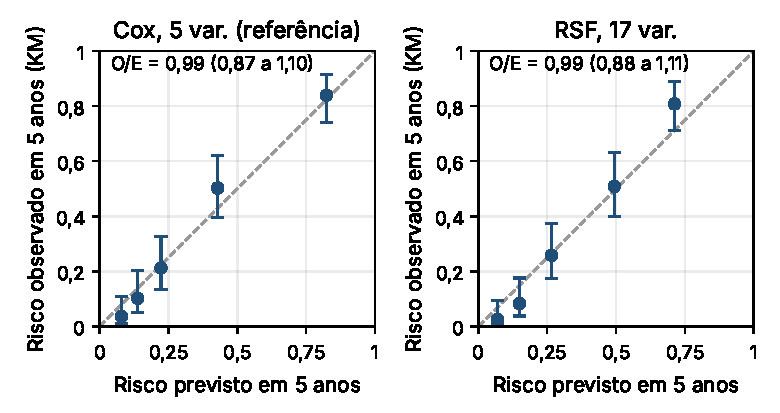
\includegraphics[height=3.2cm]{figuras/figura_calibracao.pdf}\hfill
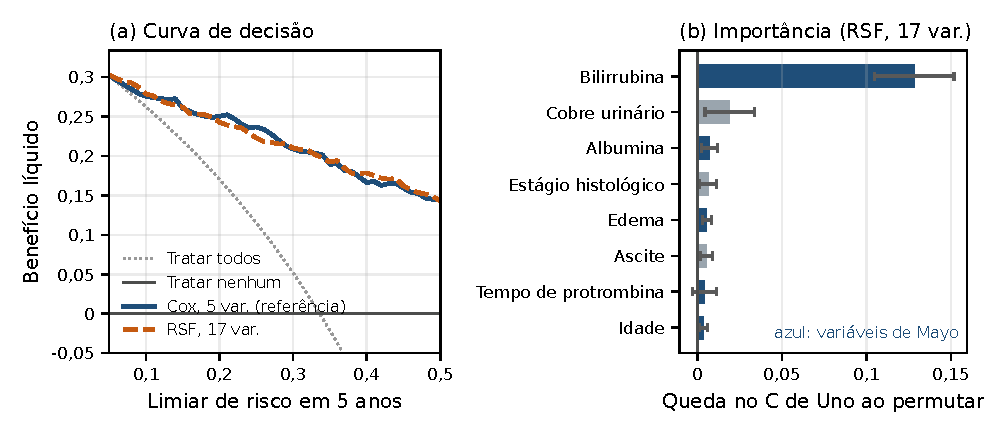
\includegraphics[height=3.2cm]{figuras/figura_decisao_importancia.pdf}
\caption{Esquerda: calibração em cinco anos por quintis de risco previsto (predições fora da partição), na referência e na RSF de maior C de Uno médio, regra fixada após a primeira execução, que introduz seleção; barras: IC 95\% do Kaplan-Meier. Direita: (a) curva de decisão em cinco anos, censura tratada por Kaplan-Meier, referência e a mesma RSF, cuja curva pode ser otimista pela seleção; (b) importância por permutação na RSF de 17 variáveis, queda média do C de Uno no teste (barras: desvio entre 5 partições), as oito maiores.}
\label{fig:painel}
\end{figure}

\subsection{Contra a fórmula de 1989 e fora do treino (análises posteriores)}\label{subsec:formula}

Contra a fórmula de Mayo publicada em 1989, sem reajuste (último bloco da Tabela~\ref{tab:leitura}), o quadro do desfecho principal se repete: o Cox reestimado ficou praticamente igual a ela (diferença de \refMenosFormula), e nenhum modelo de AM mostrou ganho demonstrado, embora a fórmula seja avaliada nos pacientes em que foi estimada; o tamanho desse favorecimento é pequeno (Tabela~\ref{tab:fontes}). No desfecho só óbito, para o qual a fórmula foi derivada, ela ficou nominalmente à frente do Cox reestimado (C de \formulaCObito{} contra \refAgrObito; diferença de \refMenosFormulaObito, com intervalo do \textit{bootstrap} sem zero, de \refMenosFormulaObitoInf{} a \refMenosFormulaObitoSup, e do teste corrigido com zero, até \refMenosFormulaObitoTcSup), e a RSF de 5 variáveis ficou abaixo dela só no \textit{bootstrap} (\rsfCincoMenosFormulaObito; \rsfCincoMenosFormulaObitoInf{} a \rsfCincoMenosFormulaObitoSup; teste corrigido até \rsfCincoMenosFormulaObitoTcSup), um indício, não uma demonstração; os outros dois modelos não diferiram dela, e em nenhum desfecho houve ganho de AM sobre a fórmula.

Nos 106 pacientes não randomizados, que nenhum modelo viu no treino, o C de Uno foi de \subUnoA{} (\subUnoInfA{} a \subUnoSupA{}) na referência, \subUnoB{} no Cox penalizado, \subUnoC{} na RSF de 5 variáveis, \subUnoD{} na de 17 e \subFormulaIni{} na fórmula inicial de 1989, que também não os viu. Os modelos de 17 variáveis ficaram nominalmente à frente (até +\subDifRefMax{} contra o Cox reestimado e até +\subDifFormMax{} contra a fórmula inicial), sem nenhuma diferença demonstrada nas comparações pareadas, com \subEventos{} eventos. O ajuste descritivo da referência (suplementar) deu evidência contra a proporcionalidade dos riscos para o tempo de protrombina (impacto preditivo não quantificado); não detectá-la nas demais não prova que valha. Na importância por permutação da RSF de 17 variáveis (Figura~\ref{fig:painel}b), a bilirrubina dominou (queda de \impBilirubin{} no C de Uno), seguida de longe por cobre (\impCopper) e albumina (\impAlbumin); da quarta posição em diante, a ordem está dentro do desvio entre partições.

\subsection{De onde vêm os ganhos aparentes?}\label{subsec:fontes}

Algumas escolhas de avaliação produzem ganho sem que o modelo melhore. A Tabela~\ref{tab:fontes} mede, nestes dados, o efeito de cada uma e separa as que mudaram o resultado das que não mudaram. Entre os contrastes em C de Uno, o maior foi avaliar o modelo nos próprios pacientes do treino: nos 312 randomizados, o C da RSF de 17 variáveis subiu \otimRSF, mais que qualquer diferença entre modelos da Tabela~\ref{tab:leitura}, medidas nos 418; o do Cox de Mayo subiu \otimCox. Usar o tempo de seguimento como entrada, um vazamento, elevou a AUROC macro de um XGBoost em \vazamentoAUROC, em outra tarefa e com outra métrica, medida na análise de classificação anterior ao plano. Já avaliar a fórmula de 1989 nos pacientes em que foi estimada, ou trocar as variáveis do comparador pelas de \cite{graf2026coxrsf}, mudou o C em poucos milésimos; a primeira dessas linhas muda também o modelo, e por isso não isola o efeito de avaliar na amostra de derivação. Na classificação de óbito em cinco anos, sem os censurados antes disso, o melhor AM tampouco mostrou superioridade (AUROC +\classifDif; intervalo de Bonferroni para \classifComparacoes{} comparações, \classifInf{} a \classifSup).

\begin{table}[!t]
\centering
\caption{Escolhas de avaliação medidas nestes dados. No primeiro bloco, cada linha muda só a condição indicada; no segundo, a linha da fórmula muda também o modelo. Entre parênteses, IC 95\% pareado ou contagem de partições. Métricas e amostras diferem entre linhas, e os efeitos não se somam.}
\label{tab:fontes}
\footnotesize
\setlength{\tabcolsep}{3pt}
\begin{tabularx}{\textwidth}{@{}>{\raggedright\arraybackslash}p{3.1cm}>{\raggedright\arraybackslash}X>{\raggedright\arraybackslash}p{1.4cm}>{\raggedright\arraybackslash}p{3.7cm}@{}}
\toprule
Fonte & Comparação & Métrica & Efeito \\
\midrule
\linhas{tabelas/fontes.tex}
\bottomrule
\end{tabularx}
\end{table}

% =====================================================================================================
\section{Discussão}\label{sec:discussao}

A resposta à pergunta do título é ``não demonstrado'', e não ``não supera''. Nas duas inferências, nenhum modelo teve ganho demonstrado sobre o Cox de Mayo reestimado, no desfecho principal nem na sensibilidade só com óbito; em análise posterior, tampouco sobre a fórmula de 1989. Mas o estudo só descarta um ganho de 0,02 para a RSF de 5 variáveis; para o Cox penalizado e a RSF de 17 variáveis, a resposta é ``não sabemos''. Essa divisão é parte do resultado e decorre do tamanho do estudo: com 132 eventos até cinco anos (186 no seguimento todo), a meia-largura dos intervalos ficou na ordem da margem (Seção~\ref{sec:resultados}). Pela regra só do plano, a RSF de 17 variáveis também teria o ganho descartado; a regra combinada, posterior, endurece a leitura em vez de afrouxá-la. Como o desenho favorece a referência (Seção~\ref{subsec:modelos}), um resultado nulo era o mais provável, e não o tratamos como prova de equivalência; ele vale para o cenário de adoção descrito, não como veredito sobre famílias de algoritmos, e é compatível, em sentido geral, com \cite{christodoulou2019systematic}.

Para além do caso, o trabalho quantifica, nos mesmos dados, quais escolhas de avaliação importam e quais não. Avaliar no próprio treino e deixar o tempo de seguimento entrar como preditor mudaram o resultado; reestimar a fórmula, trocar as variáveis do comparador ou sortear outra semente, não (Tabela~\ref{tab:fontes}). O ganho aparente de avaliar no treino foi medido nos 312 e as diferenças entre modelos nos 418, e nenhum dos trabalhos citados avalia no próprio treino: \cite{graf2026coxrsf} usa \textit{bootstrap} .632+, um estimador com correção de otimismo, e o otimismo medido aqui não explica o C de 0,855 daquele trabalho. O que a medida mostra é a ordem de grandeza do erro quando esse cuidado falta.

O contraste com \cite{graf2026coxrsf} é instrutivo. Nos mesmos 312 randomizados e com as partições deste estudo, um Cox com as sete variáveis do conjunto final daquele trabalho teve C de Harrell de \harrellGraf, praticamente igual ao do Cox de Mayo (\harrellMayo) e ao da RSF de 17 variáveis (\harrellRSF); o C de 0,776 relatado lá vem de outro protocolo (seguimento completo, \textit{bootstrap} .632+) e de um modelo que o texto não identifica, de modo que os números não são diretamente comparáveis. Com comparação pareada fora da amostra, a vantagem da RSF não aparece nestes dados. As acurácias próximas de 90\% em dados sintéticos derivados da coorte \cite{shakir2025cirrhosis,tu2025cirrhosis} tampouco são comparáveis (outro desfecho, outros dados), e procedimentos descritos nesses trabalhos, como balanceamento antes da divisão e teste nos pacientes que geraram os dados de treino, podem produzir vazamento \cite{kapoor2023leakage}.

\textbf{Limitações.} Os dados vêm de um único centro, de 1974 a 1984, antes do ácido ursodesoxicólico, e não representam os pacientes atuais; não houve coorte externa. A ponderação pela censura supõe censura independente dos preditores, não verificada. Na sensibilidade com óbito, censurar os transplantados não dá a probabilidade observável de morrer antes de um transplante, que exigiria riscos competitivos \cite{putter2007competing}. O desenho não é equilibrado (Seção~\ref{subsec:modelos}). A comparação com a fórmula de 1989, a medida das fontes de ganho aparente e a regra de leitura combinada são posteriores aos resultados, e a primeira não é cega. Por fim, a conclusão vale para os modelos e grades avaliados; na sobrevivência, não testamos \textit{boosting} nem redes neurais.

% =====================================================================================================
\section{Conclusão}\label{sec:conclusao}

Na coorte pública da Mayo Clinic, sob um plano de análise registrado antes dos resultados de sobrevivência, nem a RSF nem o Cox penalizado mostraram ganho sobre o Cox reestimado com as cinco variáveis de Mayo na predição de óbito ou transplante em cinco anos. O estudo responde ``não'' para a RSF de 5 variáveis, cujo ganho de 0,02 no C de Uno foi descartado, e ``não sabemos'' para os outros dois: a coorte é pequena demais para decidir a margem escolhida, e essa distinção é parte do resultado, que vale para um cenário de adoção que favorece a referência e penaliza os modelos de 17 variáveis pela imputação. Em análises posteriores ao plano, nenhum modelo superou a fórmula publicada em 1989, e avaliar a floresta no próprio treino produziu um ganho aparente maior que qualquer diferença entre modelos. A lição é de método: julgar o ganho do AM contra o modelo clínico pertinente à população e ao momento da predição, fora da amostra de treino, com a incerteza explícita e sem variáveis que vazem o desfecho. A continuidade natural é repetir a pergunta em coortes atuais de pacientes tratados, contra GLOBE e UK-PBC e com riscos competitivos.

\section*{Declaração de uso de inteligência artificial generativa}

Ferramentas de IA generativa foram usadas sob supervisão da autoria, que definiu a pergunta, o desenho, o plano de análise e a regra de leitura, decidiu cada desvio e interpretou os resultados. O Claude (Anthropic) apoiou a escrita do código, a execução dos experimentos e a redação. O Codex (OpenAI) auditou código e conclusões sem permissão para alterar o repositório, onde estão seus relatórios; outros agentes de IA fizeram revisões críticas e sugeriram e auditaram as análises do plano complementar; o ChatGPT (OpenAI) revisou o texto. O conteúdo final é de responsabilidade da autoria, que conferiu os números.

\bibliographystyle{sbc}
\bibliography{referencias}

\end{document}
